\documentclass[tikz,border=10pt]{standalone}
\usepackage{tikz}
\usetikzlibrary{shapes,arrows.meta,positioning,calc}
\usepackage{helvet}
\renewcommand{\familydefault}{\sfdefault}
\usepackage{xcolor}
\usepackage{varwidth}

% Color palette
\definecolor{rnaBlue}{HTML}{1F77B4}
\definecolor{tcrGreen}{HTML}{2CA02C}
\definecolor{intPurple}{HTML}{9467BD}
\definecolor{pc6Orange}{HTML}{FF7F0E}
\definecolor{softGray}{HTML}{F7F7F7}
\definecolor{grayText}{HTML}{4B4B4B}

\tikzset{
base/.style={rounded rectangle, draw=black!60, fill=white, thick, minimum width=3.6cm, minimum height=1.4cm, align=center, font=\sffamily\bfseries, inner sep=6pt},
rna/.style={rounded rectangle, draw=rnaBlue, fill=rnaBlue!6, thick, minimum width=3.2cm, minimum height=1.0cm, align=center, font=\sffamily\bfseries, inner sep=6pt},
tcr/.style={rounded rectangle, draw=tcrGreen, fill=tcrGreen!6, thick, minimum width=3.2cm, minimum height=1.0cm, align=center, font=\sffamily\bfseries, inner sep=6pt},
purple/.style={rounded rectangle, draw=intPurple, fill=intPurple!6, thick, minimum width=4.2cm, minimum height=1.2cm, align=center, font=\sffamily\bfseries, inner sep=6pt},
outbox/.style={rounded rectangle, draw=black!60, fill=white, thick, minimum width=3.6cm, minimum height=1.2cm, align=center, font=\sffamily\bfseries, inner sep=6pt},
arrow/.style={-{Latex[length=3.6mm]}, thick},
pc6bubble/.style={draw=pc6Orange, fill=pc6Orange!12, rounded corners, inner sep=5pt, font=\sffamily\small}
}

\begin{document}
\begin{tikzpicture}[every node/.style={font=\sffamily}, node distance=12mm]

% Coordinates (absolute positions give consistent spacing)
% Input
\node[base] (input) at (0,0) {Peripheral Blood\\ {\small Single-cell RNA + TCR}};

% Small cell/tube icon left of input (stylized)
\node[inner sep=0pt] (icon) at (-1.4,0) {\begin{tikzpicture}[scale=0.55]
\fill[rnaBlue] (0,0) circle (0.28);
\fill[rnaBlue!60!white] (0.65,0.18) circle (0.22);
\fill[tcrGreen] (0.35,-0.36) circle (0.24);
\draw[black!50, thin] (-0.1,-0.7) ellipse (0.45 and 0.10);
\end{tikzpicture}};

% Feature extraction branches
\node[rna] (rna) at (4,1.2) {RNA\\ {\small PCA (PC1--PC50)}};
\node[tcr] (tcr) at (4,-1.2) {TCR\\ {\small Sequence Encoding}};

% PC6 annotation bubble near PCA
\node[pc6bubble] (pc6) at (5.7,1.9) {PC6 $\rightarrow$\\Mitochondrial activity};

% Integration
\node[purple] (integr) at (9,0) {Multimodal\\ {\small Feature Matrix}};

% Model and output
\node[purple] (model) at (13.2,0) {Deep Learning\\ {\small (MLP)}};
\node[outbox] (output) at (17.6,0) {Response vs\\ {\small Non-response}};

% Arrows: Input -> branches
\draw[arrow, color=rnaBlue] (input.east) to[out=8,in=180] (rna.west);
\draw[arrow, color=tcrGreen] (input.east) to[out=-8,in=180] (tcr.west);

% Arrows: branches -> integration
\draw[arrow, color=rnaBlue] (rna.east) to[out=0,in=150] (integr.west);
\draw[arrow, color=tcrGreen] (tcr.east) to[out=0,in=210] (integr.west);

% Arrow: integration -> model -> output
\draw[arrow, color=intPurple] (integr.east) to[out=0,in=180] (model.west);
\draw[arrow, color=black!75] (model.east) to[out=0,in=180] (output.west);

% Small MLP icon left of model
\begin{scope}[shift={(11.1,0)}]
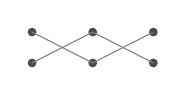
\begin{tikzpicture}[scale=0.7]
% three layers of two neurons
\foreach \x in {0,1.1,2.2}{
\fill[grayText] (\x,0.28) circle (0.08);
\fill[grayText] (\x,-0.28) circle (0.08);
}
\draw[grayText!70, thin] (0,0.28) -- (1.1,-0.28);
\draw[grayText!70, thin] (0,-0.28) -- (1.1,0.28);
\draw[grayText!70, thin] (1.1,0.28) -- (2.2,-0.28);
\draw[grayText!70, thin] (1.1,-0.28) -- (2.2,0.28);
\end{tikzpicture}
\end{scope}

% Output binary icons (Response / Non-response)
\begin{scope}[shift={(19.6,0)}]
\node[draw=none, inner sep=0pt] (r) at (0.6,0.3) {
\begin{tikzpicture}[scale=0.8]
\fill[tcrGreen] (0,0) circle (0.26);
\node[white] at (0,0) {\sffamily\bf R};
\end{tikzpicture}};
\node[draw=none, inner sep=0pt] (nr) at (0.6,-0.35) {
\begin{tikzpicture}[scale=0.8]
\fill[pc6Orange] (0,0) circle (0.26);
\node[white] at (0,0) {\sffamily\bf NR};
\end{tikzpicture}};
\end{scope}

% Subtle guiding line to indicate horizontal flow (thin, soft)
\draw[grayText!20, thin] (-0.95,0) -- (19,0);

% Legend (compact) — optional small label to indicate colors (keeps figure self-contained)
\begin{scope}[shift={(0,-2.25)}]
\node[anchor=west, align=left, font=\sffamily\small, text=grayText] at (0,0) {\textbf{Key:} , RNA (blue) ; TCR (green) ; Integrated/Model (purple) ; PC6 (orange)};
\end{scope}

\end{tikzpicture}
\end{document}